\documentclass[tikz,border=10pt]{standalone}
% No extra TikZ libraries are needed for this figure.
\begin{document}
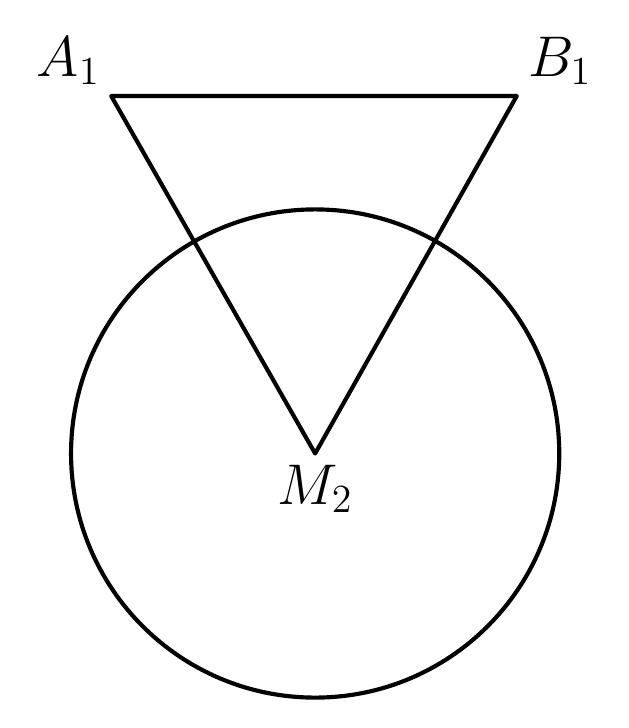
\begin{tikzpicture}[line join=round, line width=1.5pt]
  % Coordinates: s = 0.02623 cm/px, centred on the ink bbox centre (177.7, 193.5) px
  \coordinate (A1) at (-2.58,  3.82);   % px (79.4, 48.0)
  \coordinate (B1) at ( 2.57,  3.82);   % px (275.6, 48.0)
  \coordinate (M2) at ( 0.01, -0.72);   % px (178.1, 221.0), circle centre

  % Circle: centre M2, radius 118 px = 3.10 cm, full solid
  \draw (M2) circle (3.10);

  % Triangle sides: A1B1, B1M2, M2A1 (solid, no overhangs)
  \draw (A1) -- (B1) -- (M2) -- cycle;

  % Labels at the stated font size (cap height 19 px)
  \node[above left]  at (A1) {\fontsize{21}{25.2}\selectfont $A_1$};
  \node[above right] at (B1) {\fontsize{21}{25.2}\selectfont $B_1$};
  \node[below]       at (M2) {\fontsize{21}{25.2}\selectfont $M_2$};
\end{tikzpicture}
\end{document}